\chapter{Mengenal Kecerdasan Buatan dan Scikit-Learn}
Buku umum yang digunakan adalah \cite{russell2016artificial} dan  
untuk sebelum UTS menggunakan buku \textit{Python Artificial Intelligence Projects for Beginners}\cite{eckroth2018python}.
Dengan praktek menggunakan python 3 dan editor anaconda dan library python scikit-learn.
Tujuan pembelajaran pada pertemuan pertama antara lain:
\begin{enumerate}
\item
Mengerti definisi kecerdasan buatan, sejarah kecerdasan buatan, perkembangan dan penggunaan di perusahaan
\item
Memahami cara instalasi dan pemakaian sci-kit learn
\item
Memahami cara penggunaan variabel explorer di spyder
\end{enumerate}
Tugas dengan cara dikumpulkan dengan pull request ke github dengan menggunakan latex pada repo yang dibuat oleh asisten riset.

\section{Teori}
Praktek teori penunjang yang dikerjakan :
\begin{enumerate}
\item
Buat Resume Definisi, Sejarah dan perkembangan Kecerdasan Buatan, dengan bahasa yang mudah dipahami dan dimengerti. Buatan sendiri bebas plagiat[hari ke 1](10)
\item
Buat Resume mengenai definisi supervised learning, klasifikasi, regresi dan unsupervised learning. Data set, training set dan testing set.[hari ke 1](10)
\end{enumerate}

\section{Instalasi}
Membuka https://scikit-learn.org/stable/tutorial/basic/tutorial.html. Dengan menggunakan bahasa yang mudah dimengerti dan bebas plagiat. 
Dan wajib skrinsut dari komputer sendiri.
\begin{enumerate}
\item
Instalasi library scikit dari anaconda, mencoba kompilasi dan uji coba ambil contoh kode dan lihat variabel explorer[hari ke 1](10)
\item
Mencoba Loading an example dataset, menjelaskan maksud dari tulisan tersebut dan mengartikan per baris[hari ke 1](10)
\item
Mencoba Learning and predicting, menjelaskan maksud dari tulisan tersebut dan mengartikan per baris[hari ke 2](10)
\item
mencoba Model persistence, menjelaskan maksud dari tulisan tersebut dan mengartikan per baris[hari ke 2](10)
\item 
Mencoba Conventions, menjelaskan maksud dari tulisan tersebut dan mengartikan per baris[hari ke 2](10)
\end{enumerate}


\section{Penanganan Error}
Dari percobaan yang dilakukan di atas, apabila mendapatkan error maka:

\begin{enumerate}
	\item
	skrinsut error[hari ke 2](10)
	\item
Tuliskan kode eror dan jenis errornya [hari ke 2](10)
	\item
Solusi pemecahan masalah error tersebut[hari ke 2](10)

\end{enumerate}



\section{Jesron Marudut Hatuan/1164077}
\subsection{Teori}
\begin{enumerate}
\item Definisi, sejarah, dan perkembangan kecerdasan buatan.
\subitem Kecerdasan Buatan (Artificial Intelligence atau AI) dapat didefinisikan sebagai kecerdasan yang ditunjukkan oleh suatu entitas buatan. Sistem seperti ini biasanya dianggap komputer. Kecerdasan diciptakan lalu dimasukkan ke dalam suatu mesin atau komputer supaya dapat melakukan pekerjaan-pekerjan yang dapat dilakukan manusia.
\subitem Sebenarnya area Kecerdasan Buatan (Artificial Intelligence) atau disingkat dengan AI, dimulai dari munculanya komputer sekitar tahun 1940-an, meskipun sejarah perkembangannya dapat dilacak dari zaman Mesir kuno. Pada akhir tahun 1955, Newell dan Simon mengembangkan The Logic Theorist atau program AI terdahulu. Program ini merepresentasikan masalah sebagai model pohon, lalu penyelesaiannya dengan  memilih cabang yang akan menghasilkan kesimpulan terbenar. Program tersebut berdampak besar dan menjadi batu loncatan dalam mengembangkan bidang AI. Pada tahun 1956 John McCarthy dari  Massacuhetts Institute of Technology dianggap sebagai bapak AI, menyelenggarakan konferensi untuk menarik para ahli komputer bertemu, dengan  nama kegiatan The Dartmouth Summer Research Project On AI. Konferensi Dartmouth saat itu mempertemukan para pendiri dalam AI, dan bertugas untuk meletakkan dasar bagi masa depan  pemgembangan dan penelitian AI. John McCarthy  disaat itu mengusulkan definisi AI adalah AI merupakan cabang dari ilmu komputer yang berfokus pada pengembangan komputer agar mempunyai kemampuan dan berprilaku seperti manusia.
\item  Definisi supervised learning, klasifikasi, regresi, dan unsupervised learning. Data set, training set dan testing set. 
\subitem Supervised learning merupakan sebuah pendekatan dimana sudah terdapat data yang dilatih, dan terdapat variable yang ditargetkan sehingga tujuan dari pendekatan ini adalah mengkelompokan suatu data ke data yang sudah ada. Sedangkan unsupervised learning tidak memiliki data latih, sehingga dari data yang ada, kita mengelompokan data tersebut menjadi 2 bagian atau 3 bagian dan seterusnya.
\subitem Klasifikasi adalah salah satu topik utama dalam data mining atau machine learning. Klasifikasi yaitu suatu pengelompokan data dimana data yang digunakan tersebut mempunyai kelas label atau target.
\subitem Regresi adalah Supervised learning tidak hanya mempelajari classifier, tetapi juga mempelajari fungsi yang dapat memprediksi suatu nilai numerik. Contoh, ketika diberi foto seseorang, kita ingin memprediksi umur, tinggi, dan berat orang yang ada pada foto tersebut.
\subitem Data set adalah cabang aplikasi dari Artificial Intelligence/Kecerdasan Buatan yang fokus pada pengembangan sebuah sistem yang mampu belajar sendiri tanpa harus berulang kali di program oleh manusia.
\subitem Training set yaitu jika pasangan objek, dan kelas yang menunjuk pada objek tersebut adalah suatu contoh yang telah diberi label akan menghasilkan suatu algoritma pembelajaran.
\subitem Testing set digunakan untuk mengukur sejauh mana classifier berhasil melakukan klasifikasi dengan benar\cite{zhu2009introduction}.
\end{enumerate}


\subsection{Instalasi}
\subsubsection{Instalasi Library Scikit dari Anaconda}
\begin{enumerate}
\item Sediakan aplikasi Anaconda terlebih dahulu
\begin{figure}[ht]
\centerline{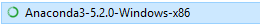
\includegraphics[width=1\textwidth]{figures/0.PNG}}
\caption{Applikasi Anaconda.}
\end{figure}
\item Setelah di install, masukkan script dibawah ini untuk melihat versi Python dan Anacondanya
\begin{figure}[ht]
\centerline{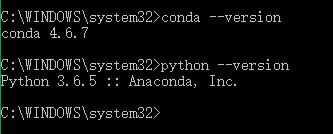
\includegraphics[width=0.75\textwidth]{figures/1.JPEG}}
\caption{Versi Anaconda.}
\end{figure}
\item  Selanjutnya masukkan perintah 'pip install -U scikit-learn'
\begin{figure}[ht]
\centerline{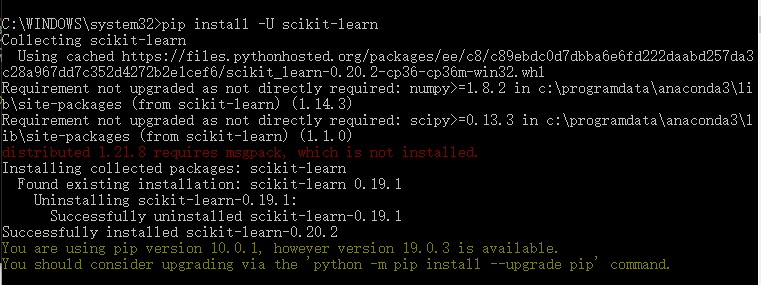
\includegraphics[width=0.75\textwidth]{figures/2.JPEG}}
\caption{Instalasi.}
\end{figure}
\item  Selanjutnya masukkan perintah 'conda install  scikit-learn'
\begin{figure}[ht]
\centerline{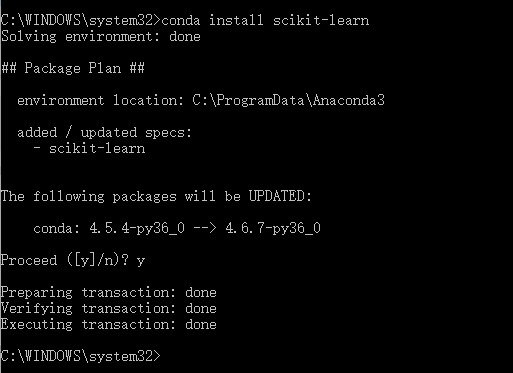
\includegraphics[width=0.75\textwidth]{figures/3.JPEG}}
\caption{Langkah installasi anaconda.}
\end{figure}
\item  Selanjutnya masukkan perintah 'python' dan 'print ('jesron')
\begin{figure}[ht]
\centerline{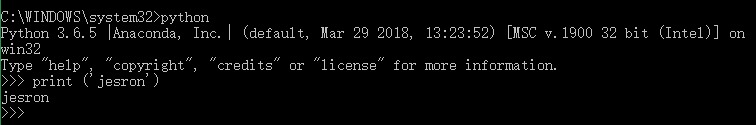
\includegraphics[width=0.75\textwidth]{figures/4.JPEG}}
\caption{Langkah terakhir.}
\end{figure}
\end{enumerate}